% 
% Author: Bratin Mondal
% Roll No: 21CS10016
% Deparment of Computer Science and Engineering
% Indian Institue of Technology, Kharagpur
%

\documentclass[12pt]{article}
\usepackage{amsmath, amssymb, graphicx}
\usepackage{amsthm}  
\usepackage{float} 
\usepackage{geometry}
\usepackage{hyperref} 
\usepackage{cleveref}
\usepackage{algorithm}
\usepackage{algorithmic}
\geometry{a4paper, top=0.25in, bottom=0.25in, left=0.25in, right=0.25in}  

\title{Computational Geometry (CS60064)\\ Homework Set 2}
\author{
    Bratin Mondal - 21CS10016
}
\date{}

\newtheorem{claim}{Claim} 

\begin{document}
\maketitle

\section*{Question 1}
For some algorithm, we have to test whether a point \( r \) lies to the left or right of the directed line \( \vec{pq} \) through two points \( p \) and \( q \). Let \( p = (p_x, p_y) \), \( q = (q_x, q_y) \), and \( r = (r_x, r_y) \).

\begin{enumerate}
    \item[(a)] Show that the sign of the determinant
    \[
    D = \begin{vmatrix}
    1 & p_x & p_y \\
    1 & q_x & q_y \\
    1 & r_x & r_y
    \end{vmatrix}
    \]
    determines whether \( r \) lies to the left or right of the line.

    \item[(b)] Show that \( |D| \) is in fact twice the area of the triangle determined by \( p \), \( q \), and \( r \).

    \item[(c)] Why is this an attractive way to implement the basic test in any algorithm where the location of a point is determined with respect to a directed line? Provide arguments for both integer and floating-point coordinates.
\end{enumerate}

\section*{Solution}

(a) We can simplify \( D \) by performing the following row operations: 
1. Subtract the second row from the third row.
2. Subtract the first row from the second row.

This gives:
\[
D =
\begin{vmatrix}
1 & p_x & p_y \\
0 & q_x - p_x & q_y - p_y \\
0 & r_x - q_x & r_y - q_y
\end{vmatrix}
\]

Expanding this determinant, we find:
\[
D = (q_x - p_x)(r_y - q_y) - (r_x - q_x)(q_y - p_y).
\]

We are working with three points \( p, q, r \) in the plane. The vector from \( p \) to \( q \) is:
\[
\vec{v} = \langle q_x - p_x, q_y - p_y \rangle.
\]

To determine which side \( r \) is on, we need the orthogonal vector to \( \vec{v} \). If a line has slope \( b/a \), the orthogonal line has slope \( -a/b \). Thus, the orthogonal vector is:
\[
\vec{v}' = \langle -(q_y - p_y), q_x - p_x \rangle.
\]

Next, we compute the dot product of this orthogonal vector and the vector from \( q \) to \( r \). If these vectors point in the same direction, the dot product is positive, indicating that \( r \) is on one side of \( q \) (left side). If the vectors point in opposite directions, the dot product is negative, indicating that \( r \) is on the other side of \( q \) (right side). If the dot product is zero, the points are collinear.

\begin{figure}[H]
    \centering
    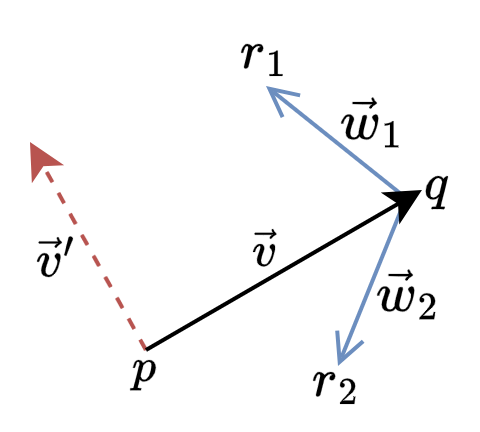
\includegraphics[width=0.3\textwidth]{img/Line_Orientation.png}
    \caption{Determining the orientation of a point with respect to a directed line. The point \( r_1 \) is on the left side of the line and \(\vec{w}_1 \cdot \vec{v}' > 0\), while the point \( r_2 \) is on the right side and \(\vec{w}_2 \cdot \vec{v}' < 0\).}
    \label{fig:line}
\end{figure}

The vector from \( q \) to \( r \) is:
\[
\vec{w} = \langle r_x - q_x, r_y - q_y \rangle.
\]

The dot product is:
\[
\vec{v}' \cdot \vec{w} = (q_x - p_x)(r_y - q_y) - (r_x - q_x)(q_y - p_y).
\]

This result is the same as \( D \), confirming the equivalence.

\vspace{0.5cm}

(b) Let \( \vec{pq} \) be the base of our triangle. Using the same notation as in part (a), this has length \( ||\vec{v}|| \) (where \( ||\vec{v}|| \) is the length of the vector \( \vec{v} \)). The height is given by the component of \( \vec{qr} \) that is perpendicular to the base, which has length:
\[
\frac{| \vec{v}' \cdot \vec{w} |}{||\vec{v}'||}.
\]

Also note that \( ||\vec{v}|| = ||\vec{v}'|| \). Therefore:
\[
|D| = |\vec{v}' \cdot \vec{w}| = ||\vec{v}|| \cdot \frac{|\vec{v}' \cdot \vec{w}|}{||\vec{v}'||} = \text{base} \cdot \text{height}.
\]

The area of the triangle is:
\[
\text{Area} = \frac{1}{2} \cdot \text{base} \cdot \text{height}.
\]

Thus:
\[
|D| = 2 \cdot \text{Area of the triangle}.
\]

This confirms that \( |D| \) is indeed twice the area of the triangle.

\vspace{0.5cm}

(c) This method is appealing due to its advantages in computational efficiency and precision. Calculating \( |D| \) involves basic arithmetic operations such as addition, subtraction, and multiplication. Notably, it does not require division operations. These arithmetic operations are computationally inexpensive and less susceptible to significant numerical errors.

For integer coordinates, these operations produce exact results since integers are represented without approximation in most computational systems. This guarantees precise calculations and eliminates concerns about rounding errors.

In the case of floating-point coordinates, while these operations remain efficient, there is a potential for minor numerical errors due to the inherent limitations of floating-point representation. Nevertheless, these errors are typically negligible when compared to the inaccuracies introduced by more complex operations, such as trigonometric or inverse trigonometric functions.

By comparison, alternative methods often involve evaluating trigonometric or inverse trigonometric functions. Such calculations are not only computationally intensive but also more prone to numerical inaccuracies.



\section*{Question 2}

Let $S$ be a set of $n$ disjoint line segments whose upper endpoints lie on the line $y = 1$ and whose lower endpoints lie on the line $y = 0$. These segments partition the horizontal strip $[-\infty, \infty] \times [0, 1]$ into $n + 1$ regions: $R_1, \dots, R_{n+1}$. Give an $O(n \log n)$-time algorithm to build a binary search tree on the segments in $S$ such that the region containing a query point can be determined in $O(\log n)$ time. Also, describe the query algorithm in full detail.

\begin{figure}[H]
    \centering
    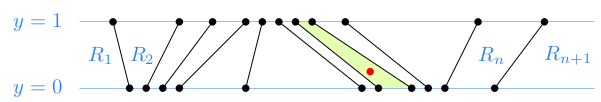
\includegraphics[width=0.5\textwidth]{img/Q2_Diagram.png}
    \caption{Determining the region of a query point in a strip.}
    \label{fig:strip}
\end{figure}

\section*{Solution}
\subsection*{Binary Search Tree Construction}
Let \( S = \{s_1, s_2, \dots, s_n\} \) denote the set of segments, where each segment \( s_i \) is defined by its upper endpoint \( u_i \) and lower endpoint \( l_i \). The segments are disjoint and non-overlapping, meaning that if \( s_i \) and \( s_j \) are two segments, then:  
\[
u_{ix} < u_{jx} \Rightarrow l_{ix} < l_{jx}, \quad \text{and} \quad l_{ix} < l_{jx} \Rightarrow u_{ix} < u_{jx}.
\]  
Here, \( u_{ix} \) and \( l_{ix} \) denote the \( x \)-coordinates of the upper and lower endpoints of segment \( s_i \), respectively.

To construct a binary search tree, we use the ordering of the upper endpoints of the segments. In our construction, each segment is stored at a leaf node of the binary search tree. Non-leaf nodes are used to guide the search for the region containing the query point. Specifically, internal nodes only direct the search towards either the left or right subtree. Any search for a query point will always terminate at a leaf node.

\subsubsection*{Sort and Build Tree}

We first sort the segments based on their upper endpoints. After sorting, the binary search tree is built recursively by selecting the median segment as the root and constructing the left and right subtrees using the segments on either side of the median. To ensure that all segments are stored in the leaf nodes, the root segment is also included in the right subtree. This process continues recursively until all segments are placed in the leaf nodes.

The time complexity for sorting the segments is \( O(n \log n) \), and the construction of the binary search tree requires \( O(n) \) time, as each segment is processed exactly once. Thus, the overall time complexity of this approach is \( O(n \log n) \).



\subsection*{Query Algorithm}

Let us denote the query point as \(q = (q_x, q_y)\). It is clear that for the query point \(q\) to lie in the strip, it must satisfy \(0 \leq q_y \leq 1\). We determine the region containing the query point by traversing the binary search tree.

Each segment \(s_i\) in the strip divides the space \([-\infty, \infty] \times [0, 1]\) into two regions: one on the left side of the segment and one on the right. Assume for now that the directions of the segments are from the bottom endpoint \(l_i\) to the top endpoint \(u_i\). 

For any other segment \(s_j\) lying to the right of \(s_i\), it holds that \(u_{jx} > u_{ix}\) and \(l_{jx} > l_{ix}\). Similarly, any segment \(s_k\) lying to the left of \(s_i\) satisfies \(u_{kx} < u_{ix}\) and \(l_{kx} < l_{ix}\). Thus, given a query point \(q\), determining its orientation with respect to the segment \(s_i\) allows us to discard all segments lying on the opposite side of \(q\). This orientation information is precisely what the binary search tree provides. 

The query algorithm is outlined as follows:

\begin{algorithm}
\caption{Query Algorithm} \label{alg:query}
\begin{algorithmic}[1]
\STATE \textbf{Input:} Query point \(q = (q_x, q_y)\), Binary search tree \(T\)
\STATE \textbf{Output:} Region containing the query point
\STATE Let \(v\) be the root of the binary search tree
\WHILE{\(v\) is not a leaf}
    \STATE Perform an orientation test of \(q\) with respect to the segment at \(v\)
    \STATE Compute the magnitude of the cross product \((u_v - l_v) \times (q - l_v)\)
    \IF{The cross product is positive}
        \STATE Move to the left child of \(v\): \(v \gets \text{left child of } v\)
    \ELSE
        \STATE Move to the right child of \(v\): \(v \gets \text{right child of } v\)
    \ENDIF
\ENDWHILE

\STATE Perform a final orientation test for \(q\) with respect to the segment at \(v\)
\STATE Compute the cross product \((u_v - l_v) \times (q - l_v)\)
\IF{The cross product is positive}
    \RETURN The region between segment \(v\) and the previous segment in the tree. (If \(v\) is the leftmost segment, return the region to the left of \(v\))
\ELSIF{The cross product is negative}
    \RETURN The region between segment \(v\) and the next segment in the tree. (If \(v\) is the rightmost segment, return the region to the right of \(v\))
\ELSE
    \RETURN The point \(q\) lies on the segment \(v\)
\ENDIF
\end{algorithmic}
\end{algorithm}

\begin{figure}[H]
    \centering
    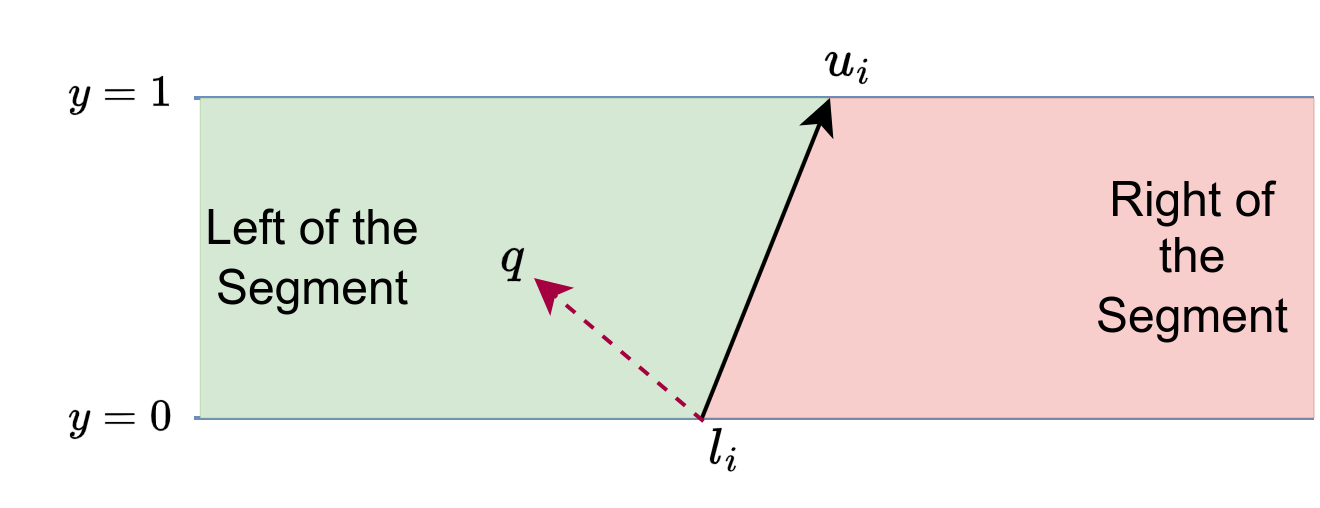
\includegraphics[width=0.5\textwidth]{img/Segment_Location.png}
    \caption{Orientation test for determining the region containing a query point with respect to a segment.}
    \label{fig:query}
\end{figure}

\Cref{alg:query} describes the query algorithm for determining the region containing a given query point \(q = (q_x, q_y)\). By leveraging a binary search tree that organizes the segments in the strip, the algorithm efficiently determines the orientation of \(q\) relative to each segment. At each step, segments lying on the opposite side of \(q\) are discarded, narrowing down the search space. The process continues recursively until the appropriate region containing \(q\) is identified. This approach ensures logarithmic complexity in the number of segments, making it computationally efficient for large datasets.

\textbf{Time Complexity:} The query algorithm has a time complexity of \(O(\log n)\), where \(n\) is the number of segments in the strip. This complexity arises from the binary search tree traversal, which efficiently prunes the search space based on the orientation of the query point with respect to each segment. The algorithm's logarithmic time complexity enables fast region determination for a given query point, making it suitable for practical applications involving segment-based spatial partitioning.


\end {document}